\documentclass{book}
\usepackage{geometry}
 \geometry{
 a4paper,
 total={170mm,257mm},
 left=20mm,
 top=20mm,
 }


\usepackage[utf8]{inputenc}
\usepackage{braket}
\usepackage{graphicx}
\usepackage{amsmath}
\usepackage{hyperref}
\graphicspath{ {./images/} }

\title{Yet Another Introduction to Quantum Computing}
\author{Thomas R Clarke}
\date{October 2022}

\begin{document}
\maketitle
\tableofcontents

\chapter{What is quantum?}


Before we can talk about quantum computing, we first have to understand the basic concepts of quantum that make it work. 

\section{Common misconceptions about quantum}
 
In science fiction *quantum* is often used to explain away a technology that seems to defy the laws of physics. In the 2018 superhero movie *Ant-Man*, the protagonist is able to become smaller and smaller until they enter the mysterious *Quantum Realm*, described as “a reality where all concepts of time and space become irrelevant”. 

If this was how subatomic physics worked, there would be no subatomic physics $^*$.

Quantum mechanics is described by the Schrödinger equation that is built on space and time. There are some differences to classical physics, the physics everyone is used to experiencing in everyday life. Quantum it is not some magical concept which allows for anything that violates classical physics to be explained away. There are however, some small but significant features of quantum mechanics that allow for the development of new technologies. 


\section{How many physicists does it take to change a light bulb?}

In the early 20th century, a German physicist (by the cool name of Max Planck) was tasked with modelling the emission of light from a filament bulb (basically a wire that gets hot enough to glow). He came up with what is known as the black body radiation spectrum. It turns out, from his model, the energy emitted by an object with a finite temperature is not emitted in a continuous spectrum. That's to say rather than all possible wavelengths of light being emitted by this bulb only certain wavelengths were allowed. This is known as a discrete spectrum. What this in turn means is that energy is emitted are chunks, or *quanta*, with a well-defined energy. We can't have energy between these chunks. It's a bit like taking the lift (elevator in American English). One can only get on or off the lift at specific heights corresponding to the floor level. Each floor is separated by a distance and the lift can go up or down in any multiple of these distances limited by the number of floors. In between those levels the doors of the lift won't open.

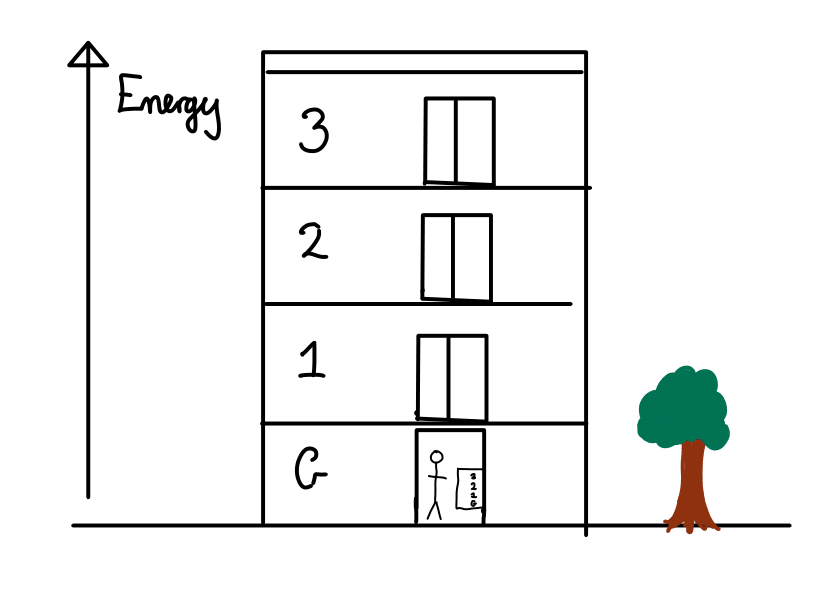
\includegraphics{images/Energy_Levels.png}

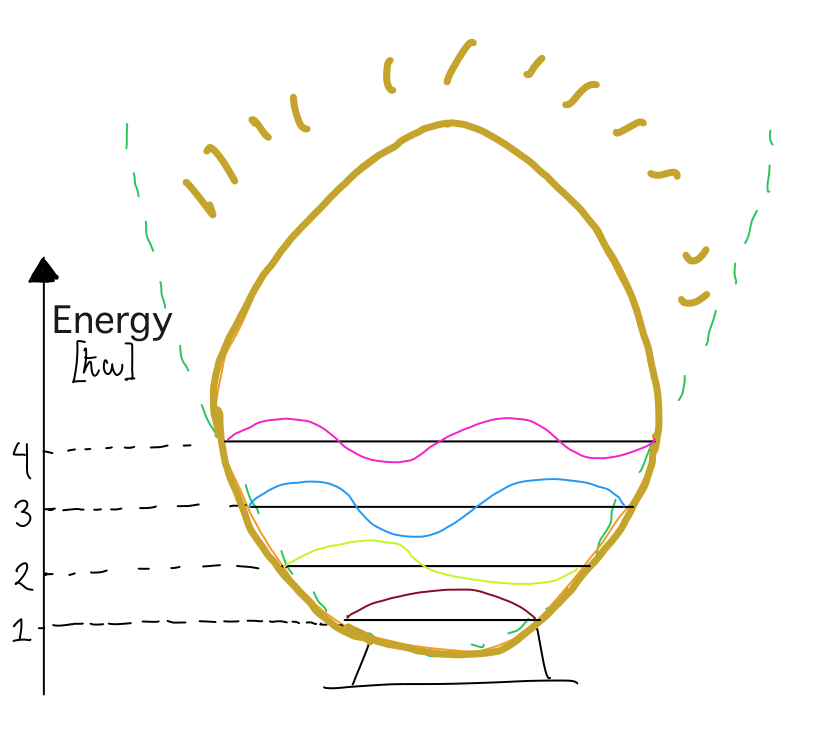
\includegraphics{images/Light_bulb_quantised.png}

This concept of quantisation of energy is where the quantum comes from. Whilst this concept is less significant to quantum computing, it is still worth mentioning. The reason for this is that the transistor that powers all digital electronics is built upon this concept. Thus all computations using this technology (the integrated circuit) are computers running on quantum mechanics. Which is not to say they are quantum computers simply that they are fundamentally built upon quantum physics, as are you, I, and everything we can see and touch. 

Beyond the quantisation of energy, there are quantum phenomena which are very much more significant to quantum computing: *superposition \& entanglement*. 

\section{So what happened to Schrödinger’s cat?}

You may have heard of a very special cat associated with another German physicist, Schrodinger. In this analogy, a cat is kept inside a black box that the observer can't view inside. Within the box, there is also a vial of poison with a radioactive source. The radioactive source has an equal probability of decaying or not decaying in some time. If the source decays, the poison is released and the cat dies. otherwise the cat is just fine. Until the observer opens the box they don't know if the cat is dead or alive. 
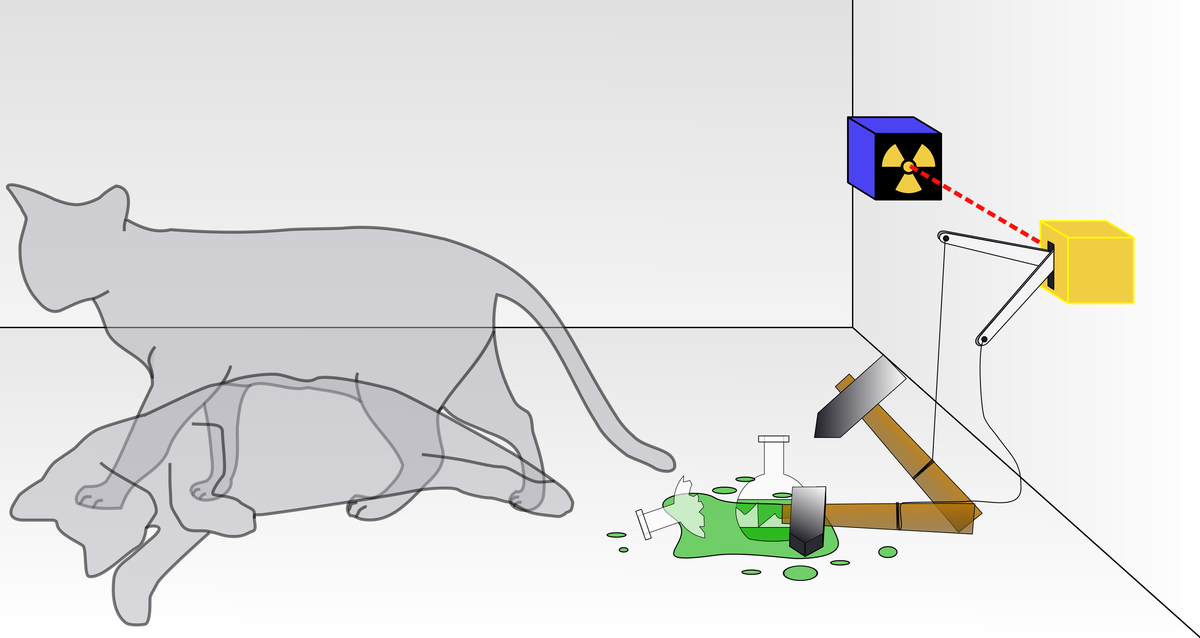
\includegraphics{images/standard_cat.png}
[2]

Schrodinger came up with this analogy to explain why quantum mechanics was so controversial for physicists that had been able to do very well with classical physics until the turn of the 20th century. This analogy is effective but is far removed from the everyday experiences one has, so another analogy can be made that encapsulates the same physics. 


<p align="center">
    It is as simple as tossing a coin.
</p>


A normal coin has two faces: heads & tails. Assuming the coin is unbiased, When the coin is tossed there should be an equal probability of landing on a heads, $P(H)$ or a tails, $P(T)$, both equal to $1/2$. Here the extremely unlikely case where the coin lands on its round edge is not considered. When the coin has not yet landed, we can say it is in a particular state where it is *like being both* heads and tails at the same time. That's not to say there are 2 coins where 1 coin is heads up and the other coin is tails facing up*. Instead this means there is some uncertainty in the state of the coin. 

In quantum mechanics we call this particular state a *superposition*. And this is the state we say the Schrodinger's cat is in before the box is opened. 

When the coin lands, it faces either heads or tails up. Now there is no uncertainty in the state of the coin. If we were to cover the coin and then look at it again some time later, it would still have the same side facing up. The superposition the coin was in before has been collapsed. The concept of looking at the coin, or opening the box, is what in quantum mechanics is known as *performing a measurement*.

$*$ According to the many worlds interpretation of quantum mechanics it is not quite so simple...

\section{Not so spooky action at a distance}

The more conceptually difficult phenomena quintessential to quantum computing can also be explained using coins (but with one small modification). For this example 2 coins will be required. 

Tossing two unbiased coins is effectively the same as tossing the same coin twice and recording the outcome each time. Guessing whether the coin is H or T is 50% for each coin or 25% for getting both of them correct. 

For the next step some removable adhesive will be required. Imagine placing the coins together with each coin having the H facing outwards and the T's stuck together to make one coin twice as thick. Tossing this coin will always result in one coin with the H facing upwards. But before the coin is revealed, the two coins are separated. The coin at the bottom must have its T side up, leaving 2 coins one H and the other T. After shuffling the coins they are separated. 

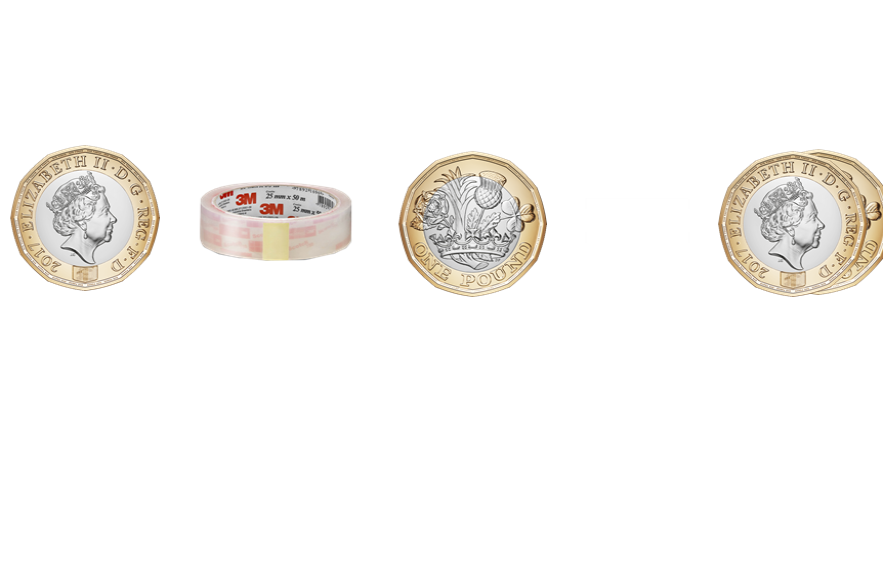
\includegraphics{images/Entanglement.png}

At this point, guessing either of the coin would have a 50\% chance of getting the right outcome- the same as for two coins tossed separately. 

But if only one of the coins is revealed, say the H coin, then it is instantly known that the other one must be a T. Suddenly guessing the state of the second coin has a 100\% chance of success whereas with the separate coin tosses revealing one made no difference to guessing the other. These linked probabilities is what is known as an *entangled state*.

\section{Quantum Technology}

Quantum Technologies, as they are defined by John Morton, director of UCLQ (as of the time of writing) are *"ones which exploit quantum superposition and entanglement to achieve major advances over current technologies in areas including communication, sensing and information processing."*

These are devices that take advantage of the aforementioned phenomena for practical applications to do something better than what can be done without using them. Quantum computation is one of the most exciting quantum technologies even if it is much less mature than others like quantum metrology (sensing) and encryption (communications).


\section{Chapter 1 Summary} 

\begin{itemize}

    \item The word quantum comes from quantised or in discrete units 
    \item A superposition happens when there are two possible states
    \item Entanglement happens when the outcomes of two individually random systems are correlated very strongly 
    \item Quantum technologies use superposition \& entanglement in their operation 
    
\end{itemize}

\chapter{What is Quantum Computing?}


In the previous chapter, the fundamental concepts of quantum mechanics were demystified and their relevance to quantum computing was explained. Building on that, this chapter will explain how quantum computers can unlock real-world value.

\section{What computers do}

Before we add quantum spice to our computers, it would be wise to first describe what it is that our classical computers do. 

Computers work by executing logical operations (think addition/subtraction/multiplication/...) that take the machine from a starting point to a finishing point. The starting point that is fed into the computer is congenitally known as the input and what the computer ends up with is usually referred to as the output. An *algorithm* is a set of instructions that allow the computer to take the input and generate an output. For example, an algorithm for doubling a number could take an input of 3, multiply it by 2 and return an output of 6. 

Going back to the coins here, this is a bit like laying them out in a row and then proceeding to shuffle and flip the coins according to a script that allows something to be done. For example, you could add 2 numbers expressed in binary by following a simple series of rules that allows for addition. This is similar to using an abacus as a calculator. Since the advent of the digital computer in the 1940's, these operations have been carried out by increasingly advanced machines to do more complex computations a lot faster.

\section{More than flipping coins} 

The example of coins being flipped can be helpful in explaining how quantum effects behave but it would not be practical to use coins for quantum computation. There are a few obvious reasons for this: 

- Flipping coins is not very fast. Modern computers have clock speeds in the GHz or billions of complete clock cycles per second. We would need an astronomical number of coins to try and replicate that. 

- Tossing coins can only really be used to generate random numbers. Beyond the conventional deterministic computing operations we can already do, the only real advantage from quantum theory would be the 'random' nature of the coin flips. 

- Sticking coins together is even slower than just flipping them. Not to mention the part where they get shuffled in a pseudo random way. 


These coins represent the qubits in a quantum computer. We should be able to control these qubits faster and more precisely than with coins:

- Perform operations on qubits quickly 
- Have a precise control over the probabilities 
- Be able to effectively control multiple qubits at once 

\section{Quantum Algorithms} 

 Conventional computers are really great at what they do. The field of high-performance computing has had many decades to mature. According to Top500, an index tracking the most powerful supercomputers, the most powerful supercomputer, Fugaku is a \$1bn powerhouse. It consumes 29,899 kilowatts to power 7,630,848 cores. For context, a mid-range laptop today might have 6 cores and consume a total of around 20 watts of power. 

 Both the laptop and the supercomputer execute algorithms that take some inputs and generate outputs. Whilst they are both excellent at solving a great many problems, there are two things they can't handle so well: superposition & entanglement. 

 Starting with a simple coin toss there are 2 possible outcomes. If we add a second coin there are 4 possible outcomes (HH, HT, TH, TT). As more and more coins are added, the number of possible outcomes doubles with each coin that is added. This number $N$, grows as $N = 2^n$. If we had 300 coins, that would mean a single toss has more possible outcomes than we estimate the total number of atoms in the universe. That's roughly 2 followed by 90 0's different combinations of H & T. Now imagine tossing these coins 300 times...

 A quantum computer could handle this problem easily. Instead of needing a universe of atoms, 300 qubits *of sufficiently high quality* would be enough to run a quantum algorithm that could simulate these coins (including sticking of them together) to arbitrary precision. 

 Quantum algorithms are similar to the input and output of classical algorithms but with the addition of superposition and entanglement in the middle.  If an algorithm doesn't feature superposition & entanglement, it would always be better to use the classical computer. 


\emph{Quantum computers are \textbf{not} faster versions of regular computers}

\emph{ Quantum computers are \textbf{not} used to run conventional algorithms, or do things that are already very well done on a classical computer }

\section{Quantum Advantage} 

If our conventional computers perform so many tasks better, there must be some motivation for quantum computing being such an exciting area of research. Aside from the elegance of manipulating quantum states, quantum computing is expected to be more useful than a glorified coin tossing simulator. Despite the limitations in state-of-the-art quantum computing machines, it is known of a few valuable applications where quantum algorithms *theoretically outperform* the best available classical solution.

> Quantum advantage occurs when a quantum computer gives significant benefit to the user compared to the best available classical alternative. 

There are a few different ways a quantum computer could add value: 

\begin{itemize}
    \item Solve a problem faster for better decision making
    \item Provide more accurate solutions that are more useful 
    \item Consume less energy and thus cost less to run 
    \item Enable entirely new models & solutions to solve problems that previously couldn't be solved
\end{itemize}

    

Quantum advantage is described in terms of how the solution scales with the size of the problem. As the problem becomes bigger and more complicated, the time taken for the computer, classical or quantum, to find a solution increases. If there is a speedup for a quantum algorithm, there is some 

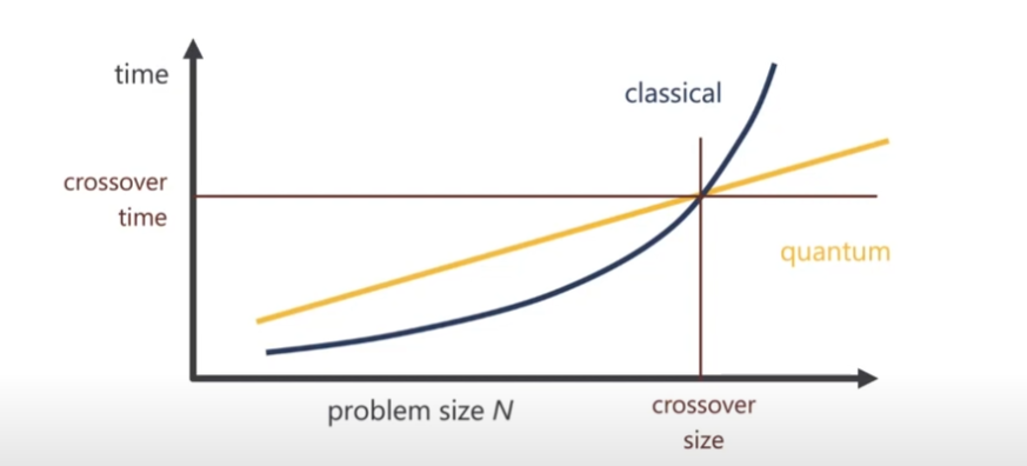
\includegraphics{images/Q_advantage.png}

As of the time of writing, there has been no practical demonstration of a problem with real world (outside physics) problem where using a quantum computer was better than using the best classical solution. As quantum computers become increasingly powerful it is hoped that this threshold will be crossed in the next few years...


\section{Applications of Quantum Computing}

There are a great many practical difficulties in implementing QC. Even still, in 2021 \href{https://www.mckinsey.com/business-functions/mckinsey-digital/our-insights/quantum-computing-funding-remains-strong-but-talent-gap-raises-concern}{over \$3 billion was invested into quantum computing}. Why is there so much hype around such an early-stage technology? 

There are many industries expecting significant value creation from quantum computing: 

\begin{itemize}
        
    \item Pharmaceuticals: Develop better medicine by simulating drugs more quickly & accurately  
    \item \hyperlink{https://www.youtube.com/watch?v=jA7iopqDm94}{Supply chain & logistics}: Quantum computing to optimise supply chains 
    \item Finance: Portfolio optimisation & fraud detection by simulation of stochastic variables
    \item Environmental: Simulation of chemistry for batteries, solar cells & materials
    \item Science: Simulation of quantum systems to better understand the universe
    
\end{itemize}


Across each of these areas, there are multiple established companies and start-ups developing quantum solutions. It is expected that the combined value creation by 2030 will be in the \$10's of billions. 

In addition to potential direct impacts, there are a lot of potential benefits to developing the hardware. Being able to measure qubits better can help develop quantum sensors with applications in healthcare & navigation. 


\section{} Chapter 2 Summary 

- Quantum computers are more than just random objects that have superposition
- Algorithms are sets of instructions that we give a computer to process information 
- Quantum algorithms are like conventional algorithms but they allow us to use superposition & entanglement 
- For some applications, quantum algorithms have shown to be much better than classical algorithms
- When a quantum computer completes a task better than the best available classical solution, there is quantum advantage

\chapter{The Mathematical Minimum for QC}
\section{Complex Numbers}

So far everything in this textbook has been described using *real* numbers- that is the set numbers you can produce on most calculators. For quantum computing, we require going beyond to complex numbers. You may be wondering why we need imaginary numbers. The most important equation in all of quantum mechanics, the Schrodinger equation, features imaginary numbers. 

$$ i\hbar \frac{\partial{}}{\partial{t}}\ket{\psi} = \hat{H}\ket{\psi} $$

Where $i = \sqrt{-1}$, $\hbar$ is the reduced Planc constant, $\hat{H}$ is a special operator called the Hamiltonian, and $\ket{\psi}$ is the statevector for the quantum system. 

This equation describes how quantum systems change with time. Whilst it is very important for quantum mechanics, it is not needed for this introductory course. Neither will there be any calculus.

\subsection{ The square root of -1}

There are two square roots of $4$: $+2$ \& $-2$. For numbers that aren't integers there are algorithms we can run on our calculators to work out the roots to arbitrary precision. In physics there are many situations in which the only valid solution to an equation calls for the square root of a negative number. To make this work, it is necessary to first define the square root of $-1$ as $i = \sqrt{-1}$. 

Using some basic algebra we can factorise any surd (square root number) into a product of two surds $ \sqrt{ab} = \sqrt{a} \times \sqrt{b}$. This holds true for negative numbers allowing us to take the square root of any negative number by breaking it down into the square root of $-1$ and the positive magnitude of that number. This can be written as:

$$ \sqrt{-a} = \sqrt{-1} \times \sqrt{a} $$

$$ \sqrt{-a} = \pm i \sqrt{a} $$
For example the square root of $-4$ can be written as $+2i$, $-2i$.
These numbers that can be written as $ai$ are known as imaginary numbers. 

\subsection{ Complex numbers}

Imaginary numbers work similarly to the real numbers everyone uses on a  daily basis. One can divide, multiply, add & subtract them just as you can for real numbers. What this also means is that any of $ \div ,\times, +, - $ operations can be applied to a combination of both real and imaginary numbers. For instance, the positive root of $-4$, $2i$ can be added to $3$ as $3 + 2i $. Any such number that can be written as a sum of a real and imaginary number is called a *complex number*. More generally we can define this mathematically as:

$$ z = a + ib $$

Where $a$ and $b$ are purely real numbers. The real part of $z$ is known as $ Re(z) = a$ and similarly the imaginary component of is $ Im(z) = b$. 

\subsection{ The Argand Diagram}

Complex numbers can be represented on a graph by splitting them into their real & imaginary parts. In the Argand diagram the x axis represents the real part and the y axis represents the imaginary part. 

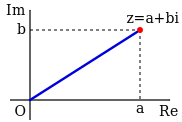
\includegraphics{images/A_plus_bi.svg}

If a were negative, the real part would be negative so the arrow would point to the left instead. If b were negative, the imaginary part would be negative, so the arrow would point downwards instead. 

\hline
\subsection{Exercise 3.1}

Consider the complex numbers 

$$ z = 4 + 5i , y = -3 + i $$

i.What is $Re(z)$? 
ii. What is $Im(m)$? 


$$m = -2 - 2i $$ 
iii. Sketch z,y,m on the Argand diagram 

\hline

\subsection{ Complex conjugate}

Every complex number has a real & imaginary part. By taking the imaginary part of the complex number and making it negative, we get the complex conjugate. For example if the complex number $z$ is 

$z = x + iy$ 

The complex conjugate would be $z^*$ written as 

$z^* = x - iy$ 

In the figure below the complex number $z$ is shown along with its complex conjugate. In this diagram $\bar{z}$ is used rather than $z^*$ but it means the same thing.  

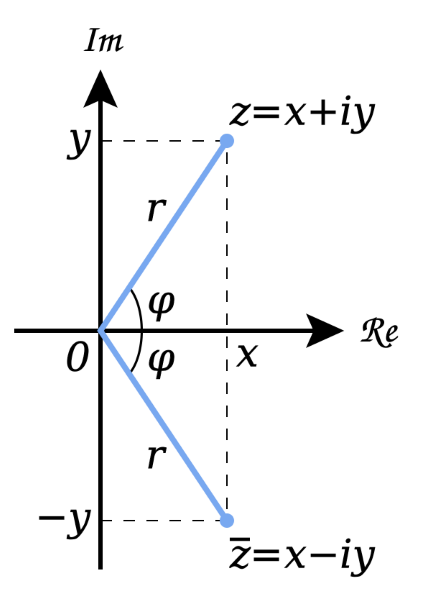
\includegraphics{images/Complex_conjugate_picture.svg.png}
 [3]

 Note how the real part is the same, but the imaginary part is on the negative axis. 

 \subsection{ Magnitude of complex numbers }

 It can be very useful to describe how big a complex number is. Since it has a real component and an imaginary component, the magnitude of a complex number indicates how big it is across both these components. 

 The magnitude of a complex number $z$ is denoted by two vertical bars as $|z|$. It is calculated the same was as the Euclidean distance as 

 $$|z| = \sqrt{x^2 + y^2}$$

 With $z = x + yi$. 

 The magnitude of a complex number is important for figuring out the probability of getting an output from a quantum computation. This will be explored in the next chapter.

> \subsection{}Exercise 3.2 

\begin{question}[subtitle=This is the Name of the first Exercise,ID=Q1]

\end{question}
>
> Consider the complex number $z = 3 + 5i$ . 
>
> i. What is the complex conjugate of $z$, $z^*$?
> 
> ii. What is the magnitude of $z$?
>
>iii. What is the magnitude of $z^*$?

\subsection{ Interlude on Trigonometry } 

Trigonometry is defined as "*the branch of mathematics dealing with the relations of the sides and angles of triangles and with the relevant functions of any angles*" but for our use it is much better to consider trigonometry the study of rotations. In later chapters, quantum gates will be described as rotations. 

Consider a circle with radius 1. Any point on the circle can be reached by rotating on the surface by an angle. The figure below shows how we can reach any point.

![Unit_circle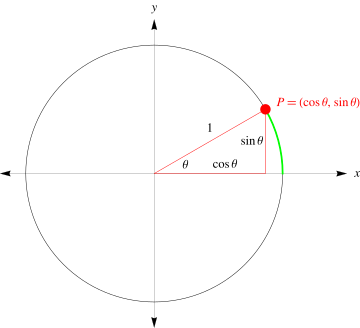
\includegraphics{images/TrigonometryUnitCircle_700.png}
[2]

The point P is reached by the angle $\theta$. It has coordinates $x = \cos(\theta)$ and $ y = \sin(\theta)$.

In chapter 5, quantum gates will be described in terms of rotations around a higher dimensional sphere. 

\subsection{}3.2.5 Euler's formula

*Euler's formula* is very useful and can be stated as:

$$ e^{i \theta} = cos(\theta) + i sin(\theta) $$

Where $\theta$ is an angle in radians. 

The significance of this is that one can represent any complex number in this fashion simply by multiplying the left-hand side by some magnitude. 

For example, the complex number $ z = \frac{1}{2}( 1 + \sqrt{3}i)$ 

Can be written as 

$$ z = cos(\pi/3) + i sin(\pi/3) $$

With Euler's formula this becomes 

$$ z = e^{i \pi/3} $$

In the context of quantum information this object $ e^{i\theta}$ is called a phase and is of exceptional importance. To explain why $\theta$ is so significant would require its own chapter. Instead it shall be incorporated into later chapters as needed.


\subsection{}3.2.6 Polar form of complex numbers 

We can represent any complex number on the **Argand diagram** in terms of its real and imaginary parts. From trigonometry, we can also represent any point on a circle using an angle and a given radius. 

Euler's formula allows us to put these two together, representing any complex number as a point on a circle. 

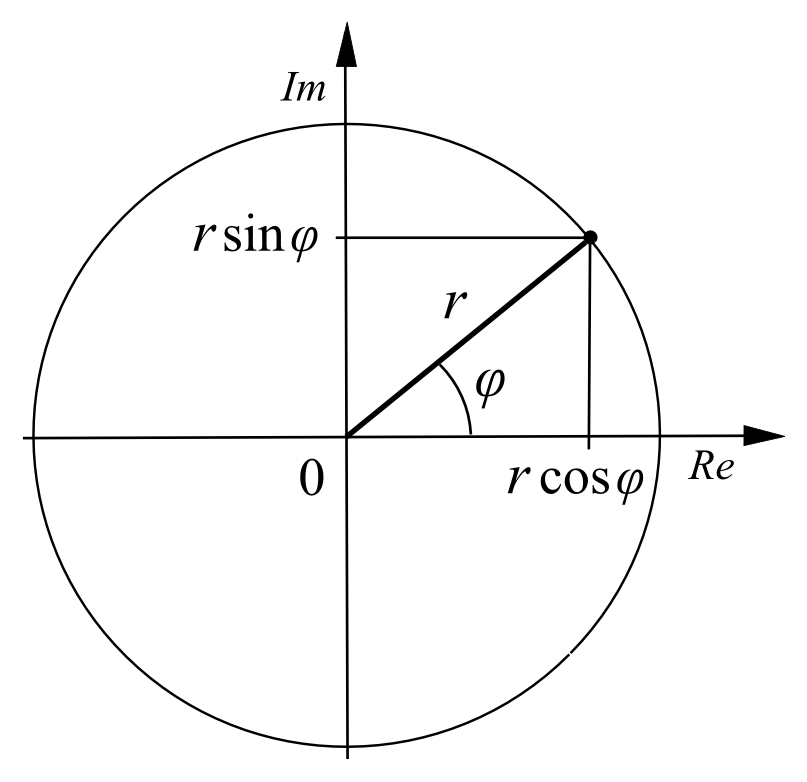
\includegraphics{images/Polar_Argand-diagram.png}
[4]

There are some complex numbers that are too big to be written as $e^{i\theta}$. For instance, the complex number z = 5 + 12i cannot be written as $cos(\theta)$ because $cos(\theta)$ only goes up to 1. To overcome this, we can multiply by some magnitude to allow for bigger numbers. By multiplying by 13 we can write 

$$ z = 13(cos(1.176) + i sin(1.176) )= 5 + 12i $$

$$ z = 13e^{i 1.176}$$

Where did the 13 come from? 

The factor in front of the $e$ is the magnitude of the complex number. This is the same magnitude described in 3.2.5. This is found by taking the norm of the real and complex part 

$$ 13 = \sqrt{ 5^2 + 12^2} $$


Using Euler's formula, any complex number can be written in terms of its magnitude and an angle. This gives us 

$$z = x + iy = re^{i\theta}$$ 

Where $r$ is the magnitude of the complex number $r = |z| = \sqrt{x^2 + y^2}$ and $\theta$ is the angle made between the real and the imaginary plane



\section{Linear Algebra}

# 3 Part 2 Linear Algebra

The second part of chapter 3 will cover linear algebra. Linear algebra is the framework for quantum computing, so it is very important to be familiar with. 

Like trigonometry, linear algebra underpins most of physics, engineering and computer science. Its importance is difficult to overstate. In 1939, Paul Dirac reformulated quantum mechanics using linear algebra [1]. Linear algebra is so important that this way of describing quantum mechanics is known as matrix mechanics. There are two key elements to linear algebra: vectors and matrices. 

\subsection{ Vectors}

Vectors are objects that have both direction & magnitude. Velocity is a vector because it has a magnitude, the speed at which the object travels with, and a direction, where it's moving towards. We will use a different notation to represent a vector with a straight line and an angled bracket as $ \ket{v} $ .

Imagine a car travelling diagonally across a road. At the same time, the car is travelling along the direction of the road as well as perpendicularly across the road. It can be said that the velocity of the car has a component pointing along the road and another component across the road. 

What makes vectors useful to work with is the fact that a vector has components. These are the individual magnitudes of the vector in each direction. We can encode the speed of the car along the road ($v_{alon}$)and the speed of the car across the road ($v_{acro}$) in a vector with two components: 

$$
\ket{v} = \begin{bmatrix}v_{alon} \\ v_{acro}
\end{bmatrix}
$$

Here the vector $\ket{v}$ has two components, $v_{alon}$ & $v_{acro}$ so the vector has a dimension of 2. In 3D space, any point can be described by 3 vectors. In general, a vector can be of any dimension, with any number of components. 

We can write any n-dimensional vector as

$$
\ket{v} = \begin{bmatrix} v_0 \\ v_1 \\ \vdots \\ v_{n-1} \end{bmatrix}
$$

Where the subscript $v_i$ indicates the i $^{th}$ component of $\ket{v}$. 

*Important note:* We start counting from 0 and end at $n-1$. This convention of counting from 0 is widely used in QC and conveniently is also used in python too. 

\subsection{ Adding vectors }

It can be useful to add vectors. All this requires is adding the corresponding components of each vector. Adding two vectors, $\ket{a}$ & $\ket{b}$

$$\ket{a} + \ket{b} = \begin{bmatrix} a_0 \\ a_1 \\ \vdots \\ a_{n-1} \end{bmatrix} + \begin{bmatrix} b_0 \\ b_1 \\ \vdots \\ b_{n-1} \end{bmatrix}
$$

The same can be done in reverse, a vector can be split into different components. For example 

$$
\ket{a} = \begin{bmatrix} 3 \\ 2 \end{bmatrix} = \begin{bmatrix} 3 \\ 0 \end{bmatrix} + \begin{bmatrix} 0 \\ 2 \end{bmatrix}
$$

This can be useful for expressing a vector in terms of its components. 

\subsection{ Multiplying a vector by a scalar }

Vectors can be made smaller or bigger by enlarging them by some scale factor. To make a vector bigger by some scale factor, the vector is multiplied by a scalar. To scale the vector $\ket{v}$ by some scalar quantity, $a$, this would be done by multiplying each component of the vector by the scalar factor. 

$$
a \ket{v} = a\begin{bmatrix} v_0 \\ v_1 \\ \vdots \\ v_{n-1} \end{bmatrix} = \begin{bmatrix} a \times v_0 \\ a \times v_1 \\ \vdots \\ a \times v_{n-1} \end{bmatrix} 
$$

>\subsection{}Exercise 3.3
>
>Imagine the vector $\ket{v}$ given by 
>
>$$\ket{v} = \begin{bmatrix} 2 \\ 1 \end{bmatrix}$$
>
>i. What is the $0^{th}$ component of $\ket{v}$ ? What about the $1^{st}$ component?
>
>ii. Write $\ket{v}$ in the form 
>
>$$
>\ket{v} = a\begin{bmatrix} 1 \\ 0 \end{bmatrix} + b \begin{bmatrix} 0 \\ 1 \end{bmatrix}
>$$
>
>iii. Write down the vector $5\ket{v}$ and describe what has changed to the vector

\subsection{ The inner product  }

It can be very useful to compare two vectors by measuring how aligned they are. Imagine two vectors pointing the same way. These two vectors would have a lot in common, and so would be perfectly aligned. The measure of how similar two vectors are is the inner product. The inner product can be calculated by multiplying each component of the vectors and adding them up. 

For example take the vectors $\ket{a}$ & $\ket{b}$ as 

 $$
 \ket{a} = \begin{bmatrix} 1 \\ 2 \end{bmatrix} ;  \ket{b} = \begin{bmatrix} 3 \\ 1 \end{bmatrix} 
 $$

 The inner product between them is $\braket{a|b}$. This can be computed by taking the column vector $\ket{a}$ and turning it into a row vector where every element of $\ket{a}$ has taken the complex conjugate. 

 $$
\braket{a|b} = \begin{bmatrix} 1^* & 2^* \end{bmatrix}  \begin{bmatrix} 3 \\ 1 \end{bmatrix}
 $$

Here the 1st component of $\bra{u}$ is multiplied by the 1st component of $\ket{v}$ and the second component of of $\bra{u}$ is multiplied by the second component of $\ket{v}$.

$$
= (1 \times 3) + (2 \times 1) = 3 + 2 = 5 
$$

This gives a scalar quantity from two vectors and is used to indicate how aligned they are. The figure below shows this, where the length of $\ket{a}$ shows the component of $\ket{u}$ in the direction of $\ket{v}$. This is then scaled by the length of $\ket{v}$ to give the inner product . 

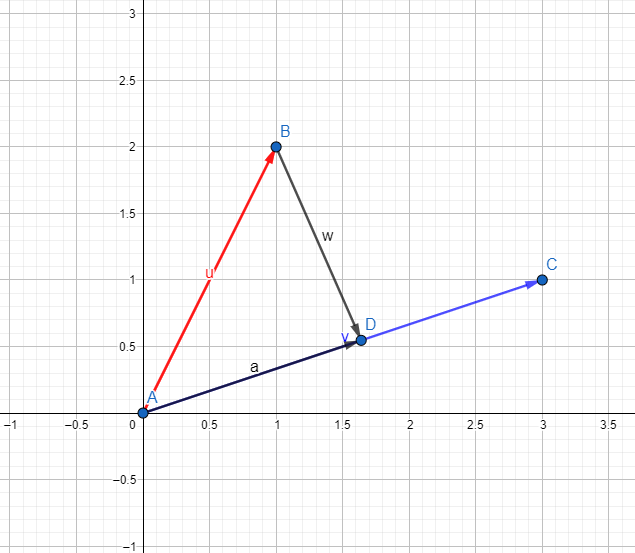
\includegraphics{images/Dot_product_visualisation.png}


The inner product depends on the angle between the vectors. If the vectors are pointing the same way, it will be bigger, if the vectors are pointing in completely opposite directions, it will be smaller. 

\subsection{ Perpendicular vectors }

If two vectors have no components in common, their inner product will be zero. This can be shown by two vectors that have an angle of $90\degree$ between them.  We call these vectors perpendicular. In quantum mechanics, the preferred term is *orthogonal* which means the same thing but applies to more than just vectors. 

For example the vectors $\ket{p} = \begin{bmatrix} 1 \\ 0 \end{bmatrix}$ & $\ket{q} = \begin{bmatrix} 0 \\ 1 \end{bmatrix}$ have a inner product  of 0. 

$$ \begin{bmatrix} 1^* & 0^* \end{bmatrix}  \begin{bmatrix} 0 \\ 1 \end{bmatrix} = (1 \times 0) + (0 \times 1) = 0$$



>\subsection{}Exercise 3.4 
>
>Let the vector $\ket{q}$ be given as 
>
>$$ \ket{q} = \frac{1}{4} \begin{bmatrix} -3 \\ 4 \end{bmatrix} $$
>
>i. Using $\ket{v}$ from the last exercise, compute 
>
>$$ \ket{y} = \ket{v} + \ket{q} $$
>
>ii. Compute the inner product $ \braket{q | v} $
>
>iii. Compute the inner product $ \braket{v | q} $ 
>
>iv. Bonus question: Compare your answers for ii. & iii. Explain any differences, if any, or why there is no difference. Does this hold for all pairs of vectors?
>
>v. Using the result from either ii. or iii. are the vectors $\ket{v}$ & $\ket{q}$ perpendicular?


>\subsection{}Exercise 3.5
>
>Compute the inner product for the vectors 
>
>$$ \ket{w} = \frac{1}{\sqrt{2}} \begin{bmatrix} i \\ 1 \end{bmatrix} ; \ket{z} = \frac{1}{\sqrt{3}} \begin{bmatrix} \sqrt{2} \\ i \end{bmatrix}$$
>
>i. $\braket{w|z}$
>
>ii. $\braket{z|w}$
>
>iii. Bonus question: Compare i. ii. . Is the result the same as from Exercise 3.2 iv? 
>If not, what has changed?
\subsection{ Matrices}

Another object, closely related to a vector, is a matrix. A matrix is just an array of numbers which you can perform a matrix product on. All the quantum gates will be represented as matrices, so understanding how they work will be essential for quantum computations. Matrices are usually denoted by capital letters, for example $M$

$$
M = \begin{bmatrix} 1 & 2  \\ 3 & 4 \end{bmatrix}
$$

$M$ has 4 elements: 1,2,3 & 4. 

\subsection{ Matrix-vector product} 

As well as storing information, matrices can be used to transform vectors. This is done using the matrix-vector product. The matrix $M$ acting on the vector $\ket{a}$ is denoted as $M\ket{a}$. The matrix multiplication is done by multiplying the corresponding elements of $M$ & $\ket{a}$. Starting from the first row of $M$ we multiply out the elements of $M$ & $\ket{a}$ starting from the left and add them up. Let's call the transformed vector $\ket{a'}$. We can compute $\ket{a'}$ by doing the matrix-vector product of $M$ on $\ket{a}$ as


$$
\ket{a'} = M\ket{a}
$$

Explicity calculating this gives us

$$
\ket{a'} =  \begin{bmatrix} 1 & 2  \\ 3 & 4 \end{bmatrix} \begin{bmatrix} 1 \\ 2 \end{bmatrix}
$$

$$
= \begin{bmatrix} (1 \times 1) + (2 \times 2) \\ (3 \times 1) + (4 \times 2) \end{bmatrix}
$$

$$
\ket{a'} = \begin{bmatrix} 5 \\ 11 \end{bmatrix}
$$

\subsection{ Inverse matrices }

For many matrix-vector products, we can go back and get the original vector from the transformed vector. This means, if we know the transformed vector $\ket{a'}$ &  the matrix $M$ we can work out the original vector $\ket{a}$. 

To get the original vector, we do the matrix-vector product, but with the transformed vector and the inverse of the matrix. This gives us 

$$
M^{-1}\ket{a'} = \ket{a}
$$

By using our equation for $\ket{v'} = M\ket{a}$ from earlier, this gives us 

$$
M^{-1}M\ket{a} = \ket{a}
$$

Notice how $\ket{a}$ is completely unchanged from applying $M$ and then $M^{-1}$. The operation $M^{-1}M$ effectively does nothing. The same would be true if we applied $M^{-1}$ first and then $M$ as $MM^{-1}$. The general name for the "do nothing" matrix is the identity. The identity is

$$M^{-1}M = MM^{-1} = I $$

As a matrix, the identity looks like 

$$ 
I = \begin{bmatrix} 1 & 0 \\ 0 & 1 \end{bmatrix}
$$

Before we had $\ket{a'} = M\ket{a}$. And now we would like to go backwards from $\ket{a'}$ to $\ket{a}$. This is done using the inverse of $M$: $M^{-1}$

$$
 M^{-1}\ket{a'} = \ket{a} 
$$

Notice how we can take the original equation and do the matrix multiplication by $M^{-1}$ and get the same result

$$
M^{-1}\ket{a'} = M^{-1}M\ket{a} = \ket{a}
$$

$M^{-1}$ is cancelling out $M$ so that there is no effect on $\ket{a}$. The matrix that represents this "no effect" is called the identity $I$ defined by 


$$ I\ket{v} = \ket{v}$$

This gives us the important relation 


$$ M^{-1}M = MM^{-1} = I $$

\subsection{ Unitary matrices} 

For all quantum gates, an important property they have is that they are unitary. Unitary matrices have an inverse equal to their conjugate transpose (the dagger at the top).

$$ U^\dagger = U^{-1} $$

This means 

$$ U^\dagger U = U^{-1}U = I $$

The conjugate transpose is the same process as it is to turn a ket (column vector) into a bra (row vector). Take You swap the rows and the columns and then replace every imaginary number with the negative version. 

All quantum gates are unitary matrices, it is very common to see the term unitary when talking about any quantum circuit. 


\subsection{Chapter 3 Part 2 Summary }

- Vectors are a collection of numbers stored in a row or column
- Vectors can be added to each other or multiplied by a scalar
- The inner product of two vectors tells us how aligned they are
- Perpendicular (orthogonal) vectors have an inner product of 0
- Matrices are arrays of numbers that can act on vectors 
- Applying a matrix to a vector turns the vector into another vector
- Matrices can have an inverse which does the reverse of the matrix 
- Unitary matrices have an inverse equal to their conjugate transpose


\chapter{Dirac Notation}
This chapter explains a bit of the framework for quantum computing using the maths from the last chapter. It's like learning the language of quantum computing, first the grammar was introduced in chapter 3, now we are defining the words.  

\section{ Information inside a computer }

When using a computer every day, it's important to be able to extract useful information from the computer. For instance, reading emails requires being able to access the information in your inbox. 

Unlike reading emails, quantum computing works at the lowest level of the system. It would be like directly accessing the bits in a classical computer. Instead of working with bits, quantum computing works with qubits. To do anything at all with qubits, it's important to describe what state they're in. The state of a qubit is described by something known as a ket. 


\subsection{ How to describe qubits?}


How do we describe the state of our qubits? It is easy to think this would require a very complicated mechanism. For us, it is as simple as a column vector! The state of our quantum computer can be described with a __column vector known as a ket__. Because it is a state represented by a vector, we call this the __state vector__. Usually, the state of our quantum computer is given by the ket $\ket{\psi}$.

The coins still work as an example for the state vector. If the coin is heads up we can use the ket $\ket{H}$, if it's tails up it is $\ket{T}$. When the coin is spinning in the air, the superposition state (see section 1.3), this state can be represented by the state $\ket{\psi}$: 

$$
\ket{\psi} = \frac{1}{\sqrt{2}}(\ket{H} + \ket{T})
$$

Since the coin has a $\frac{1}{2}$ probability of being in either heads or tails, you might have expected to see $\frac{1}{2}$ instead of $\frac{1}{\sqrt{2}}$. The reason for this is that in quantum mechanics, a state is described with an amplitude (the number outside the ket) proportional to the square root of the probability. 

We can write out our kets as the simplest column vectors

$$
\ket{H} = 

\begin{bmatrix}
1 \\ 0
\end{bmatrix}
$$

Similarly, the tails side up can be represented by the ket

$$
\ket{T} = 

\begin{bmatrix}
0 \\ 1
\end{bmatrix}
$$

This allows $\ket{\psi} $ to be expanded as 

$$
\ket{\psi} = \frac{1}{\sqrt{2}}\left(\begin{bmatrix}
1 \\ 0
\end{bmatrix}+ \begin{bmatrix}
0 \\ 1
\end{bmatrix}\right)
$$

By adding the corresponding elements of each vector, this can be simplified to

$$ \ket{\psi} = \frac{1}{\sqrt{2}}\begin{bmatrix} 1 \\ 1 \end{bmatrix} = \ket{+}$$


> This superposition state has its own symbol, $\ket{+}$.

Instead, if there were a biased coin which had a probability of heads given by $P$, we would have a different state. The probability amplitude for $H$ is $\sqrt{P}$. The probability of getting tails would be $ P(T) = 1 - P(H)$ which gives $P(T) = 1 -P$. So our probability amplitude for $T$ is $\sqrt{1 - P}$. The state of our coin is then 

$$
\ket{\psi} = \sqrt{P}\ket{H} + \sqrt{1-P}\ket{T}
$$

We can write this as a column vector as

$$
\ket{\psi} = \begin{bmatrix}
\sqrt{P} \\ \sqrt{1-P}
\end{bmatrix}
$$



> \subsection{}Exercise 4.1 
>
>Imagine a biased coin which is three times more likely to land on tails than on heads. Write down the corresponding state vector for such a coin.


\subsection{}4.1.2 How to describe the qubits 

In general, our quantum computer can take a lot more than 2 possible outcomes. Thankfully we can just add a row to our column vector for every possible outcome. So we can describe our state in terms of each possible outcomes it can take. Our quantum computer can output any number up to some maximum.  We can write the state of any quantum computer in terms of all the possible states (numbers) we can get from it

$$
\ket{\psi} = \sum_{i = 0}^{N_1} c_i \ket{i}
$$


Where the index $i$ indicates a possible state we can observe the quantum system in. There are $N$ such possible states. Each state has a probability of being measured given by $|c_i|^2$  with $c_i$ being the probability amplitude. 

Writing this as a state vector gives us 

$$
\ket{\psi} = \begin{bmatrix} c_0 \\ c_1 \\ c_2 \\ \vdots \\ c_{N-2} \\ c_{N-1} \end{bmatrix}
$$

A little note here: to model the state of a quantum computer requires keeping track of $N$ complex numbers. That doesn't seem too bad.  But for $n$ qubits we have $N = 2^n$ complex numbers to keep track of. Just 20 qubits would have more than a million complex amplitudes to keep track of! Adding 1 more qubit to get 21 qubits gives us more than 2 million complex amplitudes. 


\subsection{ Bra: Row vectors with a complex twist }


Another important quantity to define is the row vector version of the state vector. This is called a __bra__ and is represented by $\bra{\psi}$. The big difference between normal row vectors and bras is that we always take the complex conjugate for every element of the column vector (ket). 

For instance, the state with ket
$$\ket{\psi} = \frac{1}{\sqrt{2}} \begin{bmatrix} 1 \\ i \end{bmatrix} $$

Would have a bra given by 

$$
\bra{\psi} = (\ket{\psi}^*)^T 
$$

First, all the imaginary numbers in $\ket{\psi}$ get a minus sign in front 

 $$= \frac{1}{\sqrt{2}} \left(\begin{bmatrix} 1 \\ -i \end{bmatrix} \right)^T $$

Then we transpose, shown by the $^T$, by swapping the rows with the columns. We're left with our bra

$$\bra{\psi} = \frac{1}{\sqrt{2}} \begin{bmatrix} 1 & -i \end{bmatrix} $$


In the same way, we can get the coin bras. The $\bra{H}$ is the same as the ket $\ket{H} = \begin{bmatrix} 1 \\ 0 \end{bmatrix}$ but a row vector where the imaginary part of the complex numbers are all multiplied by $-1$. Since there are no imaginary numbers in $\ket{H}$, the bra $\bra{H}$ is just the transpose of the column vector as

$$
\bra{H} = (\ket{H}^*)^T = \begin{bmatrix} 1 & 0 \end{bmatrix}
$$

Just as with the column vector, we can write a general expression for any bra

$$
\bra{\psi} = \begin{bmatrix} c_0^* & c_1^* & c_2^* & \dots & c_{N-2}^* & c_{N-1}^* \end{bmatrix}
$$


\section{ Probability of measurement}


One of the most important features of quantum computing is measurement. Whenever we do a quantum computation, we change the state of the qubits. The strange thing is that we never actually see the state itself! 

In the example with the coins, we never see two coins with opposite sides up. The superposition can't be observed directly. Instead, we perform a measurement on the qubits to get some information out of them. The measurement has outcomes with different probabilities, described by the state vector. It's like the lift analogy in Chapter 1, the lift is never observed between two floors, we only see it at the floors. We also don't observe part of the lift on one floor and part of the lift on another floor. Something has gone terribly wrong if the lift is split across multiple floors! 
. 

For the coins, one may wish to know the probability of flipping the coin and getting heads or tails up. With Dirac notation, the probability of an outcome (heads up) can be calculated using the inner product (see section 3.2.4 for a refresher on the inner product).

\subsection{ Probabilities come from the inner product}

Using the coin example, the probability of the coin ending up in the heads state $\ket{H}$ can be calculated as

$$ P(H) = |\braket{H|\psi}|^2  $$

The state we want to measure $\ket{H}$ is always on the left (in a bra) and the state we have, $\psi$ is always on the right in a ket.

First we do the inner product $\braket{H|\psi}$

$$
\braket{H|\psi} = \frac{1}{\sqrt{2}}\begin{bmatrix} 1 & 0 \end{bmatrix} \begin{bmatrix} 1 \\ 1 \end{bmatrix}
$$

$$ = \frac{1}{\sqrt{2}} (1 + 0 ) = \frac{1}{\sqrt{2}}$$

Then we get the probability by taking the magnitude and squaring 

$$ P(H) = \left| \frac{1}{\sqrt{2}} \right|^2 = \frac{1}{2} $$

Since all the probabilities of the coin landing on $\ket{H}$ or $\ket{T}$ must add to 1, for a biased or unbiased coin, it must be that $P(H) + P(T) = 1$. Let the probability of getting heads be $P$. This gives us a state of 
$$
\ket{\psi} = \begin{bmatrix} \sqrt{P} \\ \sqrt{1-P} \end{bmatrix}
$$



>\subsection{}Exercise 4.2
>
>Using the definition of the measurement probability, calculate the probability of measuring heads and the probability of measuring tails. Verify that these add to 1. 



For any quantum state, the probability of measuring it to be in the state that it is must be 1. For example, if the coin were heads up, and nothing happened to the coin, the probability of measuring heads would be 1. The probability of getting a tails would be 0. This can be verified by working out the probability of measuring tails. The probability of measuring tails $P(T)$ is still given by the same equation 

$$ P(T) = |\braket{T|\psi}|^2 $$ 

where the coin is in the state $\ket{\psi}$ = $\ket{H}$. 

$$  
\left| \begin{bmatrix} 0 & 1 \end{bmatrix} \begin{bmatrix} 1 \\ 0 \end{bmatrix} \right|^2 
$$

$$
= \left| (0 \times 1) + (1 \times 0) \right|^2 = 0 
$$


On the other hand, the proability of measuring a heads is 1. Whilst this result may seem obvious, it is worth emphasising that for any quantum state, the probability of measuring it in that state should be 1 (neglecting measurement error). This leaves us the important result

$$ |\braket{\psi|\psi}|^2 = 1 $$

Another way of thinking about this is that for any quantum system, the probabilities of finding it in each of its states must add up to 1. 

> $ \braket{\psi|\psi} = 1 $ must hold for any quantum state. 

This simplifies a lot of the maths. 

\section{ Operators }

\subsection{ A trip to the casino}

An operator is a mathematical object that acts on a ket and returns a new ket. Operators are matrices that allow us to process quantum states. This is how we do quantum computing. 

Our operators are denoted by a capital letter, such as  $O$. They act on a quantum state $\ket{\psi}$ to return a new state $\ket{\psi'}$ as 

$$O\ket{\psi} = \ket{\psi'}$$

This is just a matrix-vector product. 



In gambling, the outcome of some event results in the gambler winning or losing money. Imagine a very simple game where everytime you roll a heads you win $1, everytime you roll a tails, you lose $1. 

We can define an operator, let's call it $Z$ that encodes the winnings and loses for each coin toss. 

If we roll a heads $\ket{H}$ we should get +1, so we can encode that as 

$$
Z\ket{H} = +1 \ket{H}
$$

Where the coefficient +1 is the winnings and the final state $\ket{H}$ is what we end up with. 

Similarly for tails we lose a dollar so 

$$
Z\ket{T} = -1 \ket{T}
$$

Using the vector representation of $\ket{H}, \ket{T}$ we can write the matrix $Z$

$$ Z = \begin{bmatrix} 1 & 0 \\ 0 & -1 \end{bmatrix} $$

It turns out $Z$ is an important quantum logic gate!


We can invent another operator to perform the coin flip, we will call $F$ for now can be represented as 

$$
F =  \frac{1}{\sqrt{2}} \begin{bmatrix} 1 & 1 \\ 1 & -1 \end{bmatrix}
$$

>\subsection{}Exercise 4.3 Flip the coin 
>
>By applying the flip operator to a coin that is heads up, show that it gives us the superposition state. 
>
>Hint: compute the matrix-vector product of $F\ket{H}$. 
>
> Bonus question: what would you get if you did the same with the coin starting tails up?

\section{} 4.4 What do we expect to get?

In life there are many processes where we want to predict something. For instance, a farmer would want to know how good their next harvest would be, or a stockbroker would want to know whether or not a stock is going to go up or down in price. In those cases, the farmer is not interested in the probability of getting an exact crop yield, but wants to know what yield they should expect. Quantum mechanics allows us to calculate these expectation values.

\subsection{ Classical probability }

What would we expect to get from our coin gambling example? 

We know that half the time we will get $1, and half the time we will lose $1. 

So our expected winnings, $\braket{W}$ would be
$$
\braket{W} = \frac{1}{2} \times 1 + \frac{1}{2} \times -1 
=0
$$

We win as much as we lose, so we'd expect to get nothing. 

More generally we can write the expectation value in terms of the value of each outcome and the probability 

$$ \braket{W} = \sum_{i = 0}^{N-1} X_i \times P(i) $$

Where $X_i$ is the outcome for event $i$ with probability $P(i)$ . 

 
>\subsection{}Exercise 4.4 Expectation value
>
>For this question, we're graduating from a coin to a dice. Let's call $N$ the number on a dice. Work out the expectation value by working out the number on each dice multiplied by the probability of rolling that number. 

\subsection{ A quantum description of probability }

So far this description of probability is entirely classical, even the use of angled brackets! A quantum description is more elegant. A perceptive reader might have noticed the similarities between the probability

$$ \braket{W} = \sum_{i = 0}^{N-1} X_i \times P(i) $$

And the state vector

$$
\ket{\psi} = \sum_{i = 0}^{N_1} c_i \ket{i}
$$ 

We can even get $P(i) = |c_i|^2$ so perhaps we can express the expectation value in terms of the state vector and something that gives us the outcome for each state,$X$. 

The previous example with the \$1 gain/loss coin can be repeated with some quantum sauce. Recall the operator $Z$ that gave us the win/loss for heads and tails. We would like to work out the expected earnings. We know that we can get the amount earned $X_i$

$$ X_i (\ket{i}) = Z\ket{i}$$

Where $i$ can either be $H$ or $T$. 

And we can get the probability of getting $i$ from $\braket{i|\psi}$.

Adding up all the probabilities gives us the important result
$$
\braket{Z} = \braket{\psi|Z|\psi}
$$

We have defined the expectation value of the operator $Z$. Assuming our coin is unbiased, it has the general superposition state. We can then compute the expectation value as

$$
\frac{1}{\sqrt{2}} \begin{bmatrix} 1 & 1 \end{bmatrix} \begin{bmatrix} 1 & 0 \\ 0 & -1 \end{bmatrix} \frac{1}{\sqrt{2}} \begin{bmatrix} 1 \\ 1 \end{bmatrix}
$$
$$
= \frac{1}{2}\begin{bmatrix} 1 & 1 \end{bmatrix} \begin{bmatrix} 1 \\ -1 \end{bmatrix}
$$
$$ = \frac{1}{2} ( 1 - 1) = 0 $$ 

\section{Chapter 4 Summary }

\begin{itemize}

    \item Quantum states can be represented by column vectors 
    \item We can separate out a quantum state into orthogonal components 
    \item The number in front of the component is the probability amplitude
    \item The probability of measuring a quantum system in a given state is given by the square of the modulus of the inner product
    \item The inner product of a quantum state with itself always has magnitude 1
    \item Operators transform quantum states and are represented by matrices
    \item The expectation value for any operator, $\hat{O}$  is given by $\braket{O} = \braket{\psi|O|\psi}$
\end{itemize}


\chapter{Single Qubits}

Having covered what quantum states are, this chapter will cover qubits and how we can control them. 

\section{ The unit of information}

Having introduced some of the basic mathematics to describe quantum computing, let's get started. 

Almost all articles or news reports talking about quantum computing start off by explaining how qubits are different from classical bits. This chapter will use the maths from previous chapters to give a better description of these qubits. 

Earlier, the coin example was introduced with the heads & tails outcomes we can observe. A qubit also has 2 outcomes called $\ket{0}$ & $\ket{1}$, we can just replace $\ket{H}$ with $\ket{0}$ and $\ket{T}$ with $\ket{1}$. 

$$
\ket{0} = \begin{bmatrix} 1 \\ 0 \end{bmatrix} ; \ket{1} = \begin{bmatrix} 0 \\ 1 \end{bmatrix} 
$$

These two states are called the computational basis

Just as with the coins, our qubits can be in a superposition of $\ket{0}$ & $\ket{1}$. We can have any probability of measuring $\ket{0}$ & $\ket{1}$ (so long as all the probabilities are real positive numbers which add to 1). 



\section{ The Bloch Sphere }

Dirac notation is really useful for doing algebra with quantum states. We can model how the qubits change using vectors and calculate probabilities with the inner product. One limitation of Dirac notation is that it is difficult to visualise quantum states as it does not have a diagram to represent the state vector on. 

The Bloch sphere is a useful tool used to represent the state of a qubit. Below, the quantum state $\ket{\psi}$ is represented on the Bloch Sphere. 


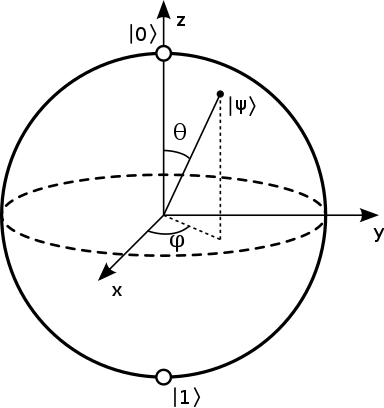
\includegraphics{images/Bloch_Sphere.png}

At the top of the sphere  is the state $\ket{0}$, at the botom is the state $\ket{1}$. Our state $\ket{\psi}$ is somewhere in between so it is a superposition of $\ket{0}$ & $\ket{1}$. The closer $\ket{\psi}$  is to the top, the greater the probability of measuring $\ket{0}$, the same is true for the bottom with $\ket{1}$. The angle $\theta$ between the $\ket{0}$ & $\ket{\psi}$ gives us these probabilities. 

Notice how $\ket{0}$ and $\ket{1}$ are seperated by $180\degree (\pi)$ on the sphere, but they are perpendicular, so the angle between them is actually $90\degree (\pi/2)$. The angles on the Bloch sphere are twice as large as the angles for the qubits.

> The angle $\theta$ on the Bloch sphere gives the probabilities with angle $\theta/2$ 

$$
P(\ket{0}) = |\braket{0|\psi}|^2 = (\cos{\theta/2})^2
$$
Similarly for the probability of $\ket{1}$

$$P(\ket{1}) = |\braket{0|\psi}|^2 = (\sin{\theta/2})^2$$


The z-axis is where the $\ket{0}$ & $\ket{1}$ are, for that reason the z-axis is known as the computational basis. In addition we have the x & y axis which correspond to different states. 

A useful tool for understanding the Bloch sphere [can be found here](https://javafxpert.github.io/grok-bloch/)


>\subsection{}Exercise 5.1: Where on the sphere
>
>We know the superposition state $\ket{+}$ has equal probabilities of $\ket{0}$ & $\ket{1}$. Where on the Bloch sphere would this state be represented? What is the angle $\theta$ that would describe this state?

\section{It's not just a phase!} 

To show probabilities, a single angle is enough. So why do we need a sphere? 

There is another important parameter that describes a qubit: the phase. 

At last, our coins will not work to describe phase, there is no analogue in classical computing, nor in probability.

Two quantum states can have the same probabilities, but be completely different states.

For example, earlier the flip coin operator $F$ had this form:

$$
F =  \frac{1}{\sqrt{2}} \begin{bmatrix} 1 & 1 \\ 1 & -1 \end{bmatrix}
$$

In quantum computing, this operator is known as a Hadamard gate with symbol $H$. 

If we apply $H$ to $\ket{0}$ we get the superposition state 

$$
H\ket{0} = \frac{1}{\sqrt{2}} ( \ket{0} + \ket{1}) = \ket{+}
$$

Applying it to $\ket{1}$ gives us a different superposition state: 

$$
H\ket{1} = \frac{1}{\sqrt{2}} ( \ket{0} - \ket{1}) = \ket{-}
$$

We call this state $\ket{-}$ because of the minus sign between the $\ket{0}$ & $\ket{1}$

The probability of getting $\ket{0}$ or $\ket{1}$ is the same for both. If we were to measure either state, we would get 0 half the time and 1 the other half the time. Since the measurement gives the same outcome you might think they are the same state. 
 
They are different states, and suprisingly there is an easy way for us to tell which one we have. 

What happens if we apply $H$ on these states? 

$$ H\ket{+} = H \frac{1}{\sqrt{2}} ( \ket{0} + \ket{1})$$

$$= \frac{1}{\sqrt{2}} (H\ket{0} + H\ket{1})$$

$$ = \frac{1}{\sqrt{2}}\left( \frac{1}{\sqrt{2}}(\ket{0} + \ket{1})+\frac{1}{\sqrt{2}}(\ket{0} - \ket{1}))  \right)$$

The $\ket{1}$'s cancel each other out and the $\ket{0}$ add together to give us

$$ = \ket{0} $$

So if we apply $H$ once to $\ket{0}$ we get $\ket{+}$ and then applying it again goes back to $\ket{0}$. 

This implies applying $H$ twice does nothing. $H^2 = I$.

So if we ever have $\ket{+}$ we apply $H$ and get $\ket{0}$ 100\% of the time. If we get $\ket{1}$ we must have had another state to begin with. If we had $\ket{-}$ would measure 1 100\% of the time. 


>\subsection{}Exercise 5.2 Back to the start
>
>Apply $H$ twice to $\ket{1}$ and verify the state we end up with is $\ket{1}$. 

>\subsection{}Exercise 5.3 The coin doesn't work
>
> When we apply the Hadamard twice to a state, we get the same state back. Without doing any maths, consider throwing a coin. Why does throwing the coin twice not guarantee you get back the side you started with?


In this example, where is the phase? 

The phase is contained in the + or - sign between the $\ket{0}$ & $\ket{1}$. 

The phase can be more than just $\pm 1$, it can be any complex number with magnitude 1. In general, any quantum state can have a phase $\phi$ 

$$ \alpha\ket{0} + \beta e^{i\phi}\ket{1} $$

With $ 0 \leq \phi < 2\pi $

We can use what we know from the Bloch Sphere to write $\alpha$ & $\beta$ in terms of the angle $\theta$


$$ \cos{(\theta/2)}\ket{0} + \sin{(\theta/2)} e^{i\phi}\ket{1} $$


Remember Euler's formula (section 3.1.2) which allows us to convert from the exponential to the complex number

$$ e^{i \phi} = cos(\phi) + i sin(\phi) $$

If we choose $\phi = 0$ we get $e^0 = 1$ which gives us 

The phase is also shown on the Bloch sphere. In the above diagram the state $\ket{\psi}$ is described by two angles $\theta$ describing the probabilities of measuring 0 or 1 and $\phi$ describing the phase. The angle $\phi$ corresponds to a rotation by $\phi$ around the z-axis in the Bloch sphere.  

Phases can be used to encode information, such as with the quantum Fourier transform, or to mark out quantum states (as with Grover's algorithm). 

> Phases only matter when they are relative. This means a phase difference between the different states. 

\section{Qubit gates }

As mentioned in Chapter 4, operators are what allow us to do things to quantum states. Below are a collection of the most common single qubit operators. 


Gate | Description| Effect on $\ket{0}$| Effect on $\ket{1}$ | Matrix 
----- | ----- | ----- | ----- | -----|
$I$ | Identity: do nothing | $\ket{0} \rightarrow  \ket{0} $ | $\ket{1} \rightarrow \ket{1}$ | $\begin{bmatrix} 1 & 0 \\ 0 & 1 \end{bmatrix}$
$X$ | Not: Swaps $\ket{0}$ with $\ket{1}$   |$\ket{0} \rightarrow \ket{1}$ |$\ket{1} \rightarrow  \ket{0}$ | $\begin{bmatrix} 0 & 1 \\ 1 & 0 \end{bmatrix}$|
$Y$ | Y: Rotation by angle $\pi$ around the y-axis of the Bloch sphere | $\ket{0} \rightarrow  i\ket{1} $ |$\ket{1} \rightarrow -i\ket{0} $ | $\begin{bmatrix} 0 & -i \\ i & 0 \end{bmatrix}$|
$Z$ | Z: Adds a phase of $e^{i\pi}$ to $\ket{1}$|$\ket{0} \rightarrow \ket{0}$|$\ket{1} \rightarrow -\ket{1}$ |$\begin{bmatrix} 1 & 0 \\ 0 & -1 \end{bmatrix}$ |
$H$ | Hadamard: Creates the superposition state | $\ket{0} \rightarrow \frac{1}{\sqrt{2}} ( \ket{0} + \ket{1})$ | $\ket{1} \rightarrow \frac{1}{\sqrt{2}} ( \ket{0} - \ket{1})$ | $\frac{1}{\sqrt{2}}\begin{bmatrix} 1 & 1 \\ 1 & -1 \end{bmatrix} $
$S$ | Adds a phase of $e^{\pi/2}$ betweeen $\ket{0}$ & $\ket{1}$|$\ket{0} \rightarrow  \ket{0} $ |$\ket{1} \rightarrow e^{i\pi/2}\ket{1}$  | $\begin{bmatrix} 1 & 0 \\ 0 & e^{i\pi/2} \end{bmatrix}$
$T$ | Adds a phase of $e^{\pi/4}$ betweeen $\ket{0}$ & $\ket{1}$ | $\ket{0} \rightarrow  \ket{0} $| $\ket{1} \rightarrow e^{i\pi/4}\ket{1}$ |$\begin{bmatrix} 1 & 0 \\ 0 & e^{i\pi/4} \end{bmatrix}$

Sometimes it is easier to perform gates by knowing what they do to the $\ket{0}$, $\ket{1}$ states, sometimes it is easier to do the matrix multiplication. 

A more comprehensive list of gates [can be found here](https://raw.githubusercontent.com/qiskit-community/qiskit-textbook/main/content/ch-states/supplements/single-gates-cheatsheet.pdf) 

> \subsection{}Exercise 5.4 
> 
> By considering the effect on $\ket{0}$ & $ \ket{1}$, or by doing matrix multiplication, calculate the following states:
>
> a. $ XZ\ket{1}$
>
> b. $ XH\ket{+} $
>
> c. $ XYZ\ket{0} $


\subsection{Aside: gates vs operators}

In the last chapter, operators were introduced as matrices that act on a quantum state. In this chapter, it seems quantum gates do the same thing. This is true, all quantum gates are operators, but not all operators are quantum gates. 

For instance, the creation operator $\hat{a}^\dagger$ creates a photon from the vaccuum but can't be represented by a matrix. The momentum operator $\hat{p} = -i\hbar\frac{\partial}{\partial x}$ is a partial derivative. 


\section{Parameterised quantum gates }

In addition to these fixed quantum gates, there are quantum gates we can specify ourselves. These gates are described by a parameter we can control to change what the gate does. These gates are very similar to nodes in a neural network where we can change the weights (we will see a lot more about these in a chapter on quantum machine learning).

For instance, we might want to get more than a 50\% chance of measuring an output. We can see on the Bloch sphere that if we rotate our quantum state by some angle towards $\ket{0}$ or $\ket{1}$ we can boost the probability of measuring those. The matrix that does this rotation is known as $R_x$

$$
R_y(\theta) = \begin{bmatrix} \cos(\theta /2) & -\sin(\theta /2) \\ \sin(\theta /2) & \cos(\theta /2) \end{bmatrix}
$$

> The angle we give as input is $\theta$ the angle we perform the rotation is $\theta/2$.

We also have rotations for the x & y axis too. In fact, the X,Y gates are special cases of $R_x(\theta)$ & $R_y(\theta)$ with $\theta = \pi$. 

$R_z(\phi)$ (also known as P) is also useful because it allows us to give any phase to a qubit. 

$$
R_z(\phi) = P(\phi) = \begin{bmatrix} 1 & 0 \\ 0 & e^{i\phi} \end{bmatrix}
$$

This gives a phase shift of $\phi$ between $\ket{0}$ & $\ket{1}$


> \subsection{}Exercise 5.5 
> By using $\theta = \pi/2$ apply $R_y(\pi/2)$ to the state $\ket{1}$. What gate does $R_y(\pi/2)$ do? 
 
> \subsection{}Exercise 5.6 
> The X gate turns $\ket{0}$ to $\ket{1}$ and $\ket{1}$ to $\ket{0}$. By considering angles on the Bloch sphere, what is the angle $\theta$ such that $R_y(\theta) = X$


\section{ The Universal Quantum Gate }

Just as we can represent any single qubit state with two parameters, we can also represent any single qubit gate using parameters. 

$$
U(\theta, \phi, \lambda) = \begin{bmatrix} \cos(\theta/2) & -e^{i\lambda}\sin(\theta/2) \\ e^{i\phi}\sin(\theta/2) & e^{i(\phi + \lambda)}\cos(\theta) \end{bmatrix} 
$$

Just as we can reach any point on the Bloch Sphere with $\theta$ & $\phi$ we can get any quantum gate using $U$. 

The set of all gates that can be made from $U$ are known as $SU(2)$. 

>\subsection{}Exercise 5.7 
> Which gate in the list above is represented by  $U(\theta, \phi, \lambda) = U(0,0,0)$ 


\section{ Bonus: Beyond Bits }

For this course, we work with qubits- 2 level quantum systems. There is considerable research into using more than 2 levels for quantum computation. Such systems are called qudits- d-level quantum systems that we can use to process quantum information. 

Qudits are much less commonly used than qubits for a few reasons

- Having multiple levels is much more complicated. Think about the X gate, for a qudit, this gate becomes much more complicated

- Qudits present even more engineering challenges than qubits. For instance, a qubit in a trapped ion consists of the ground level and the first excited state. Higher energy levels have smaller gaps in energy, so they are more difficult to control precisely. 

- Quantum error correction for qudits is much more complicated. With qubits $\ket{0}$ can only go to $\ket{1}$ but for a 4 level system there are 3 possible states it could go to. And that's just one qudit.


\section{Chapter 5 Summary }

\begin{itemize}
    \item 
    \item The state of a qubit can be represented on the Bloch sphere
    \item The BS shows the probability and phase of a qubit 
    \item The phase of a qubit is the $e^{i\theta}$ difference between the $\ket{0}$ & $\ket{1}$ states
    \item There are many qubit gates we can use to perform operations on qubits
    \item Some qubit gates are rotations specified by a parameter which describes what the gate does
    
\end{itemize}

\section{References}

[1] Chetan Wake, 2019, Introduction to quantum computing part -1 Representation of qubit using Bloch sphere


\chapter{Multiple Qubits}

\section{ More than the sum of its parts}

If quantum computing was nothing more than a collection of qubits processed individually, there would be little point in building a quantum computer. A single qubit can be modelled using 2x2 matrices - you can even work these out by hand! Even if we were to have a large number of these in parallel, it would still be very easy to simulate a large number of qubits. 

Having qubits interact with one another allows for more complex algorithms. Thanks to entanglement, one qubit can control what happens to another. This has some interesting implications for quantum algorithms. 

\section{Back to Binary }

Everyone is familiar with the decimal system where counting goes as 0,1,2,...,8,9 and then we repeat from 10,11,12,... . Computers, classical or quantum $^*$ count in base 2. 

Binary works the same way as the decimal system but instead the count repeats every 2. Numbers go as 


0,1,10,11,100,101,110,111 

Which in decimal would be 

0,1,2,3,4,5,6,7 

\subsection{ Reading binary }

To read a binary number:  
  
  
1. Count the number of digits in the number and take this number -1 as n
2. Starting from the first digit on the left, if that digit is 1, calculate $2^n$. 
3. Moving to the next digit on the right, if that digit has a 1, calculate $2^{n-1}$. 
4. Add the result of step 3 to step 2. 
5. Repeat this process for each digit decreasing the power by 1 each time until the last digit (which should have a $2^0 = 1$ calculation). 

An example of this is shown below


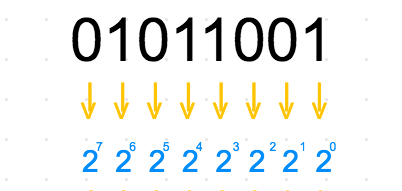
\includegraphics{Chapters/Images/binary_conversion.png}
[1]

1. Here there are 8 digits, so we take $n = 8 - 1 = 7 $. 
2. For the first digit there is a 0, so we do nothing. 
3. The second digit is 1 so we do $2^{7-1} = 2^6 = 64$. 
4. Adding $0 + 64 = 64$.
5. The sum we get is

$$
0 + 2^6 +0  + 2^4 + 2^3+ 0 + 0 + 2^0 = 89 
$$

Here we needed at least 6 digits in binary to represent a number with 2 digits in decimal. The decimal notation is much more efficient. 

>\subsection{}Exercise 6.1 
>
>What would the following numbers be in decimal?
>
>a. 1111
>
>b. 1001
>
>c. 101101
>
>d. 0110

>\subsection{}Exercise 6.2
>
>What would the following numbers be in binary? 
>
>a. 1 
>
>b. 5
>
>c.6

\subsection{ Reading quantum states }

Let's say we wanted to encode the number 5 onto a quantum state. 

We know $ 5 = 2^2 + 2^0$ so we can write 5 as 101 in binary. 

As there are 3 digits, we need 3 qubits to represent this number. 

The qubit on the left is in state 1, the qubit in the middle is in state 0 and the qubit on the right is in state 1. 

$$ \ket{101} = \ket{q_2q_1q_0} $$

Here we use the convention where the first qubit ($2^0$) is on the right, with the next qubit one to the left and the last qubit the most to the right. This is what IBM uses and what we will use when programming quantum computers.

> Quantum states are read right-to-left with the first qubit next to the >

\subsection{}6.2.3 Column vectors for multiple qubits 

Keeping with the number 5, the state vector for this number 

$$ \ket{5} = \ket{101} = \begin{bmatrix} 0 \\ 0\\ 0\\ 0\\ 0\\ 1\\0\\0 \end{bmatrix} $$

For each qubit we add, the number of rows in this column vector doubles! This is what makes it difficult to simulate quantum algorithms on classical computers. 

> \subsection{}Exercise 6.3 
> 
> For n qubits, we need a vector with $2^n$ rows to describe the state. What shape of matrix (rows, columns) do we need to describe the operator (i.e. multi-qubit gate) that acts on this vector? 


\section{ Multiple qubits, multiple gates }


If we have multiple qubits, we can apply single qubit gates on each of them at a time. This is the same as having a bunch of single qubits on their own, each having their state changed by the qubit gate. The simplest case is two qubits. Let's begin with our qubits in the normal starting state of $\ket{q_1q_0} = \ket{00}$. We can apply a Hadamard gate on the first qubit, $q_0$ to change it to the superposition state $\ket{+}$

$$ \ket{00} \rightarrow \ket{0+} $$ 

Then we might want to apply the not (X) gate to the other qubit, $q_1$ to change it to $\ket{1}$

$$ \ket{0+} \rightarrow \ket{1+} $$

As these are two seperate operations, we could do them both at the same time in one step 

$$  \ket{00} \rightarrow \ket{1+} $$

> Applying single qubit gates to a collection of qubits, changes the states of the qubits the gates are applied to


\section{ Product States }

So far we have acted on all our qubits seperately, what happens to one doesn't affect the others. If we were to measure one of the qubits, it wouldn't tell us anything about the other qubits. 

Such states where we can seperate the qubits out are called product states (or pure states). 

In general a product state can be written as 

$$ \ket{\Psi} = \ket{\psi_0}\ket{\psi_1}...\ket{\psi_{n-1}}$$

Let's say we measure the first qubit (qubit 0) and get a 0. The remaining qubits wouldn't be affected, so our new state would be 

$$ \ket{\Psi} = \ket{0}\ket{\psi_1}...\ket{\psi_{n-1}}$$


\section{ The Tensor Product }

Mathematically there is a very satisfying way of representing this with linear algebra. The tensor product allows us to do this. This is a little beyond the scope of this course, but I'll include it anwyay. 
I've been a bit lazy with notation here, is
$$ \ket{\psi_0}\ket{\psi_1} = \ket{\psi_0} \otimes \ket{\psi_1} $$
Where the symbol $\otimes$ represents the tensor product operation. 

If we use vectors to represent this it looks like 

$$ \ket{\psi_0} = \begin{bmatrix} a_0 \\ a_1 \end{bmatrix} ; \ket{\psi_1} = \begin{bmatrix} b_0 \\ b_1 \end{bmatrix} $$

$$
 \ket{\psi_0} \otimes \ket{\psi_1} = \begin{bmatrix} a_0\ket{\psi_1} \\ a_1\ket{\psi_1} \end{bmatrix}
$$

This is a new vector with $\ket{\psi_1}$ repeated twice, each time multiplied by a scalar $b_0$ or $b_1$. The final vector has 4 elements and looks like: 
$$
 \ket{\psi_0} \otimes \ket{\psi_1} = \begin{bmatrix} a_0 b_0 \\ a_0 b_1 \\ a_1b_0 \\ a_1 b_1 \end{bmatrix}
$$

So you can think of your new state as a 4-level quantum system. Every time we add another qubit, we tensor product it in, so the size of the vector doubles. This is where the exponential scaling of the state-space comes from.

The same applies for multiple quantum gates in parallel. Our matrix increases by a factor of 2 in both the number of rows or columns. This is even better scaling!

\section{ Entanglement } 

You might have noticed that it's really easy to apply single qubit gates to a collection of qubits. In the last chapter, we saw that all single qubit gates can be represented by $ 2 \times 2$ matrices. And each qubit can be represented by a column vector with 2 rows. So if we had a large number of qubits, we could still simulate a large number of $2 \times 2$ matrices on a classical computer. If it is easy to simulate a collection of isolated qubits, why do we bother making quantum computers? 

The answer comes from combining superposition with entanglement. 


\subsection{ If statements with spicy sauce }

In general programming, if statements allow you to include logic in a program. If a statement is true, the algorithm will do one thing, otherwise, if the statement is false, it will do something else. The computer first has to check the variables value before executing the next step of the algorithm. We can do this on a quantum computer by measuring our qubits, collapsing the superposition and then performing our next quantum gates accordingly. For example, [in quantum teleportation this is done](https://qiskit.org/textbook/ch-algorithms/teleportation.html). 

 For example, in section 4.3.1 there was a game where if a coin landed up we got +1 dollar, otherwise (if it were tails up) we got -1 dollars. This works as a classical if statement, provided we add the value after the coin is landed and observed. 

What makes quantum operators different is that we can apply them to the superposition. What this means is we can act on both the $\ket{H}$ and $\ket{T}$ amplitudes at once. 



Entanglement allows the superposition of one qubit to define the superposition of another

This means we can't treat our qubits as separate 2x1 vectors anymore. 


\subsection{ Can the qubit not? }

Entanglement can be created by gates that act on multiple qubits together. This can create an entangled state. The most common way this is done is by using a 2 qubit gate called the controlled-not, usually shown as CNOT or CX. The CNOT acts on two qubits, the control qubit and the target qubit. If the control qubit is in the state $\ket{0}$, it will do nothing, if the control qubit is in the state $\ket{1}$ it will perform the not (X) gate on the target qubit. In both cases, the state of the control qubit is unchanged. 

We can represent this with a table

\begin{center}
\begin{tabular}{ c c c c c}
 Control & target & $\rightarrow{}$ & control & target \\ 
 0 & 0 &  & 0 & 0 \\ 
 0 & 1 &  & 0 & 1 \\
 1 & 0 &  & 1 & 1 \\
 1 & 1 &  & 1 & 0 \\
  
\end{tabular}
\end{center}



If we have two qubits $\ket{\psi_1}_1\ket{\psi_0}_0$ where qubit 0 is in the state $\ket{\psi_0}$ and qubit 1 is in the state $\ket{\psi_1}$, there are two CNOT's we can have. One where qubit 0 is the target and qubit 1 is control or the other way around, qubit 1 is the control and qubit 0 is the target. Each of these has a different 4x4 matrix


The first has the control on the 
$$
CNOT_{0, 1} = \begin{bmatrix} 1 & 0 & 0 & 0 \\
0 & 0 & 0 & 1 \\
0 & 0 & 1 & 0 \\
0 & 1 & 0 & 0 \\
\end{bmatrix}
$$

$$
CNOT_{1, 0} = \begin{bmatrix} 1 & 0 & 0 & 0 \\
0 & 0 & 0 & 0 \\
0 & 0 & 0 & 1 \\
0 & 0 & 1 & 0 \\
\end{bmatrix}
$$


\subsection{ Ring the Bell (states)}


There are many ways we can entangle two qubits, and some qubits can be more entangled than others. The most common entangled states are known as the Bell states, and can be written like

$$ \ket{\Phi^+} = \frac{1}{2} \left( \ket{00} + \ket{11} \right) $$
$$ \ket{\Phi^-} = \frac{1}{2} \left( \ket{00} - \ket{11} \right) $$
$$ \ket{\Psi^+} = \frac{1}{2} \left( \ket{01} + \ket{10} \right) $$
$$ \ket{\Psi^-} = \frac{1}{2} \left( \ket{01} - \ket{01} \right) $$

For each of these states, we can't separate out our two qubits as a product state. 

<!-- 
The following circuit generates the Bell states

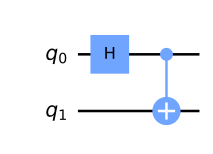
\includegraphics{Chapters/Images/Bell_State_circuit.png}


\subsection{General controlled unitaries }

Instead of having a not-gate being applied, we can have any single quantum gate. 

\subsection{Multiple-control qubit gates }

We can have controlled quantum gates where there are more than one qubit as control. In this case, the target qubit is only affected if all the control qubits are 1. 

The Toffoli gate is the same as the controlled-not gate but with two qubits needing to be 1.

\section{Chapter 6 Summary}

\begin{itemize}
    \item Quantum computers work in binary
    \item Many qubits have quantum states represented as a binary number
    \item Quantum states are read right-to-left with the first qubit at the end
    \item We can apply single qubit gates individually across multiple qubits 
    \item When qubits are independent of one another, they are in a product state
    \item When one qubit influences the state of another qubit they are entangled 
    \item We can use entanglement to apply logic gates
\end{itemize}



$^*$ There have been proposals for using a base other than 2 for quantum computing. This has some advantages but the difficulty in constructing algorithms combined with the difficulties in error correction such a device has prevented any significant machine from being built.
\section{References}

[1] L.Vivah, [Learn How to Read Binary in 5 minutes](https://medium.com/@LindaVivah/learn-how-to-read-binary-in-5-minutes-dac1feb991e), 2018

\chapter{Quantum Circuits}
\chapter{Quantum Random Number Generators}


Pick a random number between 1 and 10. 

Was it 7?    

Humans are really bad at picking random numbers. For instance, choosing 1 or 10 doesn’t seem so random because they are the largest and smallest numbers. A number picked near the middle intuitively feels more random than one at the higher or lower end. Even numbers seem less random than odd ones (though there is no reason for this to be true). 


\section{Why do we want random numbers?}

For much of human history, random numbers were only used in games of chance. Dice go back 5,000 years (Piovano, 2011/2016). During WW2, random numbers became an important statistical tool for von Neumann when he was working on the Manhattan project (Metropolis, 1987) and for use by the Germans in sending encrypted messages. 
From the Manhattan project (Metropolis, 1987) came Monte Carlo methods. These are simulations that take a large number of samples from a model using random numbers to compute something that would be difficult to solve otherwise. They are a powerful and ubiquitous tool in physics, economics and data science. It became clear that random numbers were increasingly useful in areas of science, cryptography and statistics. More recently, with the abundance of private information sent over the internet, there is considerable need to generate a large number of random numbers for various encryptions standards (Zhou & Tang, 2011).

\section{The limitations of peudorandom number generators} 


Pseudorandom number generators (PRNGs) and do not actually produce random numbers. Anyone who knows the seed (initial random number) and the algorithm can generate the entire sequence with complete certainty. If left to run for long enough, both the middle square method and linear congruential method will repeat. This is fine for videogames where it is the feeling of randomness which matters, but not so great for encrypting communications (Li, 2013). With insider knowledge of the PRNG, an attacker could decrypt the communication.

\section{Quantum RNG}

Thankfully there are ways of generating truly random numbers based on physical processes. Atmospheric noise, the cosmic microwave background (the effect that caused static on old TVs) and radioactive decay are good examples. We can measure radio wave or microwave radiation, or the number of clicks from a Geiger counter.
Quantum computers can also be used for this purpose. They are effectively controlled physical experiments leveraging quantum mechanics to perform some computation. Since randomness is an inherent part of quantum mechanics, quantum computers, unlike classical ones used by von Neumann, can serve as a True Random Number Generator (TRNG) (Jacak, 2021). This is because a quantum system can exist in a superposition of possible states, and following a measurement takes on one of these states. Whilst we can know the probability of the system taking each of these states, we cannot know with absolute certainty which it will take (Nielsen & Chuang, 2000).

Below is an example of how n random numbers (from 0 to nmax) can be generated using IBM’s quantum computer. The code creates a quantum circuit with enough qubits to represent the power of 2 greater than nmax. The qubits are then put into a superposition and measured to obtain the random number. This process is repeated 1000 times and sampled n times to produce the numbers.  

The TRNG implemented here is hardly the most practical implementation. It is rather slow, requires access to IBM’s cloud infrastructure, is vulnerable to interception, and runs on a device cooled to nearly absolute zero. A more useful implementation of this concept was done 20 years ago by the Swiss company ID Quantique, using a photonic chip. Newer models can be integrated in desktop PCs with PCIe connectivity or even USB (ID Quantique, n.d.).
\chapter{Quantum computers now and of the future}

\chapter{Quantum Algorithms}


\section{ Complexity theory isn't that complicated}

When doing a computation, we are really interested in how long it will take. How long it takes to solve a problem depends on the algorithm. If the algorithm has a lot of steps, it will take the computer longer to solve them problem. It also depends on how fast the computers is/ speed of the memory or ability to use hardware acceleration (GPUs) or parallelise the problem. 

Since the speed of the hardware varies for every computer, we prefer to consider how many steps the algorithm has. 

In computer science, complexity theory is the study of how hard problems are to solve. The hardness is described by the number of steps an algorithm needs to solve a problem.

For example, adding two n-digit numbers will require on the order of n operations. Multiplication 



\section{ Types of quantum algorithms} 


- NISQ quantum algorithms 
- Variational quantum algorithms 
    -Variational Quantum Eigensolver, Quantum Approximate Optimisation Ansatz
- Fault-tolerant quantum algorithms 
    - Shor's Algorithm, Grover's algorithm, Quantum Monte Carlo,  HHL algorithm 


\section{Fault-tolerant Quantum Algorithms} 

\subsection{ Grover's Search Algorithm}


\



## 8.5 How much do we need?

It is extremely important to keep track of the resource requirements for any quantum algorithm. 

If it turns out that an algorithm requires thousands of qubits with circuit depths in the thousands, or millions, this will not be feasable with a quantum computer in the next decade. 

Across many of the proposed quantum algorithms, significant work has been done in reducing the requirements. This can be done by making circuits more efficient- using fewer gates and fewer qubits.  It is hoped that continued progress in circuit optimisation and improved hardware specifications will allow for better quantum algorithms to be implemented in the near-term. 


\section{Practical considerations: Quantum Strategy}

- Try a small-scale proof of concept project first 
    - Small scale QC can be simulated on a classical computer. This can be a lot cheaper than buying access to an expensive QPU


- Does the problem require QC?
    - Quantum computing is a rather exotic solution proposed largely for problems tackled by supercomputers. Consider more conventional solutions before trying quantum
    - How strong is the evidence that QC has an advantage for this problem. 

- Hardware 

    - Number of qubits (is it enough to run our algorithm)
    - Quality of qubits (are the outputs reliable or just noise)
    - Pricing/ availability (can you afford it)
    - Software features/support (how user-friendly is it, is it compatible with qiksit/ML libraries, does it support optimisation of quantum circuits ect)


- Cost 
    - Currently, access to QPU time is dominated by fixed cloud overheads (i.e. the provider). This means the costs can come down very quickly as the hardware scales. 
    - Energy costs are a large part of the costs of running conventional HPC clusters. For QPU's almost all the energy requirements are in cooling (with very little in control electronics). How this scales in the future depends on the qubit type. Optimistically, energy requirements could remain fixed for the next few years as the cooling requirements are constant for a significant growth in qubit quantity & quality. 

\section{Limitations of quantum computing}

- Quantum computers are very small scale. As of the time of writing, the gate-based quantum processing unit (QPU) with the most qubits has 127 qubits. However this machine from IBM (named eagle) is not currently available for public use. At the time of writing the QPU with the most available qubits has [INSERT REFERENCE TO QPU WITH MOST QUBITS]
- Current QPU have high error rates. [INSERT FIGURE]
- Quantum computing is very expensive [Reference]

- QC is not a solution to every problem. For the vast majority of computational tasks, there is no proposed quantum algorithm. Thus, the vast majority of consumers are unlikely to benefit from QC in the medium term.


\section{Chapter 10 Summary}


\chapter{Quantum Machine Learning}

\section{Mysteries of machine learning}


In recent decades the rapid development of cheap and powerful classical processing units has transformed all aspects of society. Artificial intelligence has been pondered by humanity from as far back as the 1800's but has remained the realm of science fiction until numerous great advances in the capability of computers has facilitated many implementations of AI across various industries from medicine to the military. 

Many of these AI technologies are based on machine learning. 

\section{QC is a lot like machine learning}

There are quite a few similarities between quantum computing & machine learning. They are both:

\begin{itemize}
    \item Built on linear algebra
    \item Held back by expensive computational resource
    \item Sometimes very difficult to explain outcomes 
    \item Likely to go through period of hype & stagnation as technological development pace changes
    \item Often associated with optimisation problems 
    \item Using Python & Jupyter notebooks 
\end{itemize}


It's an open question as to whether or not quantum computing can improve machine learning. There have been some early experiments showing quantum machine learning performing better, but there have equally been experiments showing classical machine learning outperforming quantum machine learning. 

 Given the very limited number (& quality) of qubits available there haven't been any large-scale tests yet. This is likely to change in the near future...

\section{Why machine learning could benefit from a quantum advantage}

There are a few reasons motivating the use of quantum computers for machine learning:
\begin{itemize}
    \item Better sampling from true randomness of quantum states
    \item Higher dimensionality from $2^n$ dimension only requiring $n$ qubits
    \item Entanglement could be better for modelling correlations in joint-probability distributions
    \item For data generated by quantum systems can be used much [more effectively on a quantum model](https://www.science.org/doi/10.1126/science.abn7293)
\end{itemize}

\section{Variants of QML} 

\subsection{VQE}

The variational quantum eigensolver is one of the most well-known quantum algorithms. 

\subsection{QAOA}

\subsection{Generative Quantum Modelling}

\subsection{Quantum SVM} 

\section{Additional considerations}

There are quite a few things to consider with QML 
\begin{itemize}
    \item There are no proven advantages to using QML over classical ML 
    \item Quantum computers struggle to load large classical data sets 
    \item Many proposed quantum algorithms depend on quantum ram, which has yet to be scaled and integrated into QPU's. 
    \item There is significant academic scepticism, [even in companies that promote QML](https://www.youtube.com/watch?v=5UsJV2BNj2U&list=PLOFEBzvs-VvppIb0jg5_aDbmFs36DXD9w)
    \item If a classical ML solution works perfectly well for a given problem, it is much better to use that than a quantum version. 
\end{itemize}




Some optimism: 

Quantum machine learning is still a very new field. It may take quite some time to offer benefits, but that doesn't mean it isn't worth exploring.

Conventional ML doesn't have much theoretical guarantees, but we know it works really well in practice. Given there are so many diverse applications of ML, one of them is likely to be well-suited to a quantum model.

Even if our current QML approaches don't offer any value at the moment, further research may uncover models better suited to the hardware we have now...

\subsection{Additional resources for QML}

[GitHub repository listing papers, books and online courses](https://github.com/Christophe-pere/Roadmap-to-QML)  
A [panel discussion from 2021 on the Future of Quantum Machine Learning](https://www.youtube.com/watch?v=5UsJV2BNj2U&list=PLOFEBzvs-VvppIb0jg5_aDbmFs36DXD9w)

\chapter{Grover's Algorithm}

\chapter{F}

$$ N = 2^n $$
$$ \omega = e^{i2\pi /N} $$
$$F_n = \frac{1}{\sqrt{N}} \sum_{j,k = 0}^{N-1}\omega^{jk} \ket{k}\bra{j}} = \frac{1}{\sqrt{N}}\bigotimes_{j,k = 0}^{N-1}\left(\ket{0} + \omega^{}\ket{1} \right)$$



\section{The most powerful quantum subroutine}

\textit{Mathematical analysis is as extensive as nature itself; it defines all perceptible relations, measures times, spaces, forces, temperatures: this difficult science is formed slowly, but it preserves every principle which it has once acquired; it grows and strengthens itself incessantly in the midst of the many variations and errors of the human mind. Its chief attribute is clearness; it has no marks to express confused notations. It brings together phenomena the most diverse and discovers the hidden analogies which unite them.} - Joseph Fourier, The Analytical Theory of Heat (1878) 

This chapter is atypical of the rest of this textbook. Here a rather lengthy historical introduction is given in an attempt to convey the power of what could be considered the most powerful quantum algorithm. It is what drives Shor's algorithm along with every other quantum algorithm with exponential scaling. 

\section{Signal processing}

Waves surround us. Light travels from the sun to our eyes and sound travels from vibrating objects to our ears and those two waves comprise much of our experience of reality. For both light and sound, what we are sensitive to is small changes of intensity, the power per unit area, that the complex network of our sense organs and brain are able to process and interpret as what we see and hear. In engineering, signal processing is extremely important in telecommunications and in physics there are insights we can gain about the nature of solids by performing a similar analysis. In the latter two cases, the mathematics we use to accomplish these tasks is described by various Fourier Transforms. 

In 1822, French mathematician, Joseph Fourier proposed a method for 

\section{Turning the Tide}
\section{A change of perspective }
\section{The quantum mechanical treatment}

\section{Quantum Phase Estimation}
\section{The power behind Shor's Algorithm}




\chapter{Shor's Algorithm}


Probably the most famous quantum algorithm, Shor's algorithm is an example of a quantum algorithm \textit{exponentially} faster than the best classical algorithm. 

In addition to being fast, Shor's algorithm has immense practical utility. 

\section{Decrypting encryption & Y2Q}

\chapter{Distributed Quantum Computing}


\end{document}
